\section{Unit testing}
\chapterauthor{Wiktor Czetyrbok}

Without a doubt, testing is one of the essential elements in the software development life cycle. It is one of the most resource-consuming and critical stages in the application development process. A test the proper way saves you money and anguish right now, it is assuring reliability, stability, and usability all of which are fundamental for quality overall performance software. This allows you to notice and correct risks at a time you can afford to in the development cycle, which translates into lower costs and fewer failures down the line. Testing from different perspectives ensures that the software performs as intended under varying conditions, meets user requirements and validates security and performance standards.

The unit tests that we used internally to test our application, these were created in parallel with the building of new system capabilities. We used the JUnit\cite{Junit} and Mockito\cite{Mockito} libraries to create our tests. JUnit makes available a variety of assertion methods allowing to check whether the result of executing a given set of calls will be what we are expecting. A method name like \texttt{assertNotNull} (line 15, Figure \ref{fig:unit-tests}) serves as an example of this, which asserts that object is not null. Also with \texttt{assertThrows}, it is possible to verify that the right exceptions are thrown (in case of invalid data). Handling exception example can be found in the line 24 in  Figure \ref{fig:unit-tests}.

A great complement to the JUnit library is Mockito, a popular library that helps developers create mock objects. This is particularly useful for writing tests that isolate methods from the rest of the application, ensuring they are independent and don't rely on external components. To create mock objects, you annotate the fields with \texttt{@Mock}. Then, by calling \texttt{MockitoAnnotations.initMocks(this)}, Mockito automatically initializes these fields with mock objects. To define how these mock objects should behave during tests, you can use Mockito's \texttt{when} and \texttt{thenReturn} methods, which specify the expected responses when certain actions are performed. This approach allows for controlled and focused unit testing, as presented in lines 13 and 22-23 in Figure \ref{fig:unit-tests}.

\clearpage % Move the figure and everything after it to a new page

{
\label{fig:unit-tests}
\begin{minted}[linenos, frame=single]{java}
class AuthServiceTest {
    @Mock private PasswordEncoder passEncoder;
    @Mock private UserRepository userRepository;
    @InjectMocks private AuthService authService;
    @BeforeEach
    void setUp() {MockitoAnnotations.initMocks(this);}

    @Test
    void testRegister_NewCustomer_Success() {
        RegisterDTO dto = new RegisterDTO("usern", "test@ex.com", "pass");
        when(userRepository.findByEmail(dto.email())).thenReturn(empty());
        String encodedPassword = "encodedPassword";
        when(passEncoder.encode(dto.password())).thenReturn(encodedPassword);
        UserDetailsDTO result = authService.register(dto);
        assertNotNull(result);
        verify(userRepository, times(1)).save(any());
    }

    @Test
    void testRegister_ExistingCustomer_ExceptionThrown() {
        RegisterDTO dto = new RegisterDTO("user", "test@ex.com", "pass");
        when(userRepository.findByEmail(dto.email()))
        .thenReturn(Optional.of(new User()));
        assertThrows(UserAlreadyExistsException.class, 
        () -> authService.register(dto));
        verify(userRepository, never()).save(any());
    }
}
\end{minted}
\captionof{figure}{Unit tests scenarios for AuthService class.}
}
For unit testing, achieving high test coverage is crucial to ensure the reliability and maintainability of the repository. Test coverage measures the extent to which the code is exercised by the unit tests, helping identify untested or poorly tested areas. To evaluate test coverage in our Java backend service, we utilize JaCoCo\cite{JaCoCo} (Java Code Coverage), a widely used code coverage analysis tool. JaCoCo provides detailed insights into which parts of the code are being tested. By integrating JaCoCo into our \hyperref[subsec:deployment-github-actions]{CI/CD pipeline}, we ensure consistent tracking of test coverage over time and enforce quality standards during development. With over 120 test cases, in our application we managed to achieve overall coverage over 80\%, which meets modern days business standards. Bar charts visible on Figure \ref{fig:jacoco-report} and percentages display the coverage of specific java packages.

 \begin{figure}[H]
    \centering
    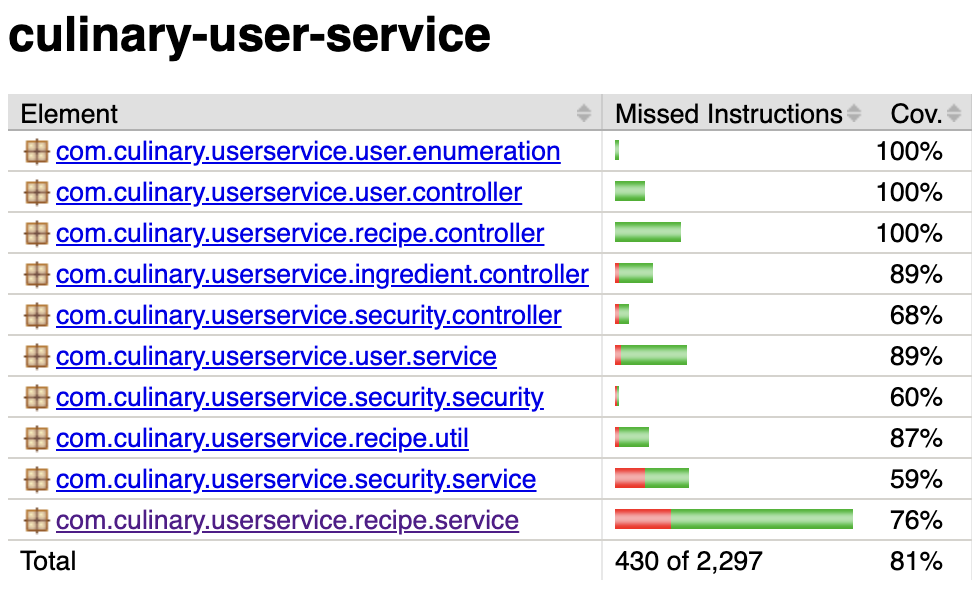
\includegraphics[width=0.8\textwidth]{images/backend-test-converage.png}
    \caption{ Jacoco test report of culinary-user-service}
    \label{fig:jacoco-report}
\end{figure}

\section{Test scenario}
\chapterauthor{Kamil Dędza}
\par
There are many different tools and techniques when it comes to testing the software. One of them is a test scenario. What is it and why is it useful? The scenario test has five key characteristics, it is (a) a story that is (b) motivating, (c) credible, (d) complex, and (e) easy to evaluate \cite{TestScenario}. For our purpose, we have created a few tasks for example users to carry out. Those are simple short stories, which are likely to occur in our system. Some of the scenarios require preconditions, meaning the expected state of the before. The scenarios contain a few simple steps. Then, after performing the steps, we can compare the predicted results with the real results that our system generated during the interaction with the user. By this assessment, the developers can see whether the solution that they have created offers required features, and that the system works well under real-life load. All scenarios were successfully completed.

\section{Test Scenarios for the "Foodies" Application}

\subsection{User Login Functionality}

Objective: \\
To ensure users can log in successfully with valid credentials and receive appropriate feedback for invalid login attempts.

Actors Involved: \\
- End User: Anna Koper (example user) \\
- System: Foodies application

Preconditions: \\
- The user has an active account on the Foodies platform. \\
- The application is available and accessible. \\
- The user's account credentials (email and password) are known and valid.

Test Steps: \\

1. Access the Login Page: Navigate to the Foodies application login page. Verify that the login form is visible, with fields for email and password, and a "Login" button. \\

2. Enter Valid Credentials: Input the correct email address in the "Email" field (e.g., \texttt{aniakoper@gmail.com}). Input the correct password in the "Password" field (e.g., \texttt{SecurePass123}). \\

\begin{figure}[H]
    \centering
    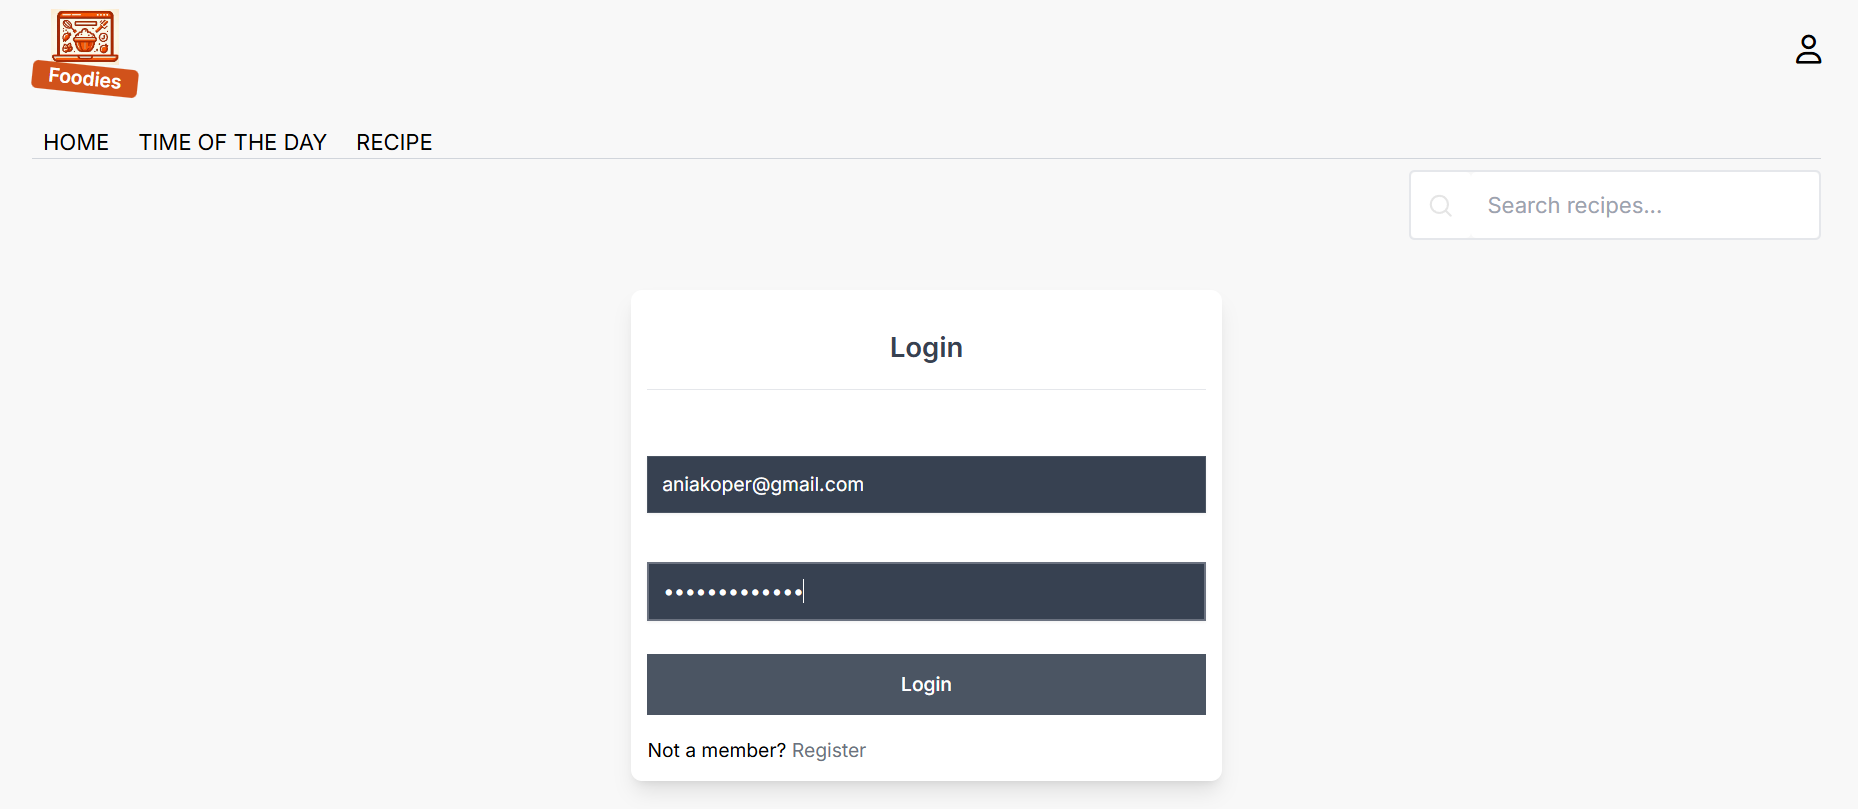
\includegraphics[width=\textwidth]{meta/pdf_attachments/images/image1.png}
    \caption{Login Page}
    \label{fig:image1}
\end{figure} 
3. Submit Login Form: Click on the "Login" button and wait for the system to process the request. \\

4. Validate Successful Login: Verify that the user is redirected to the home page. Check for the availability of user-specific data (e.g., favourite recipes, profile, modifications, settings). \\

\begin{figure}[H]
    \centering
    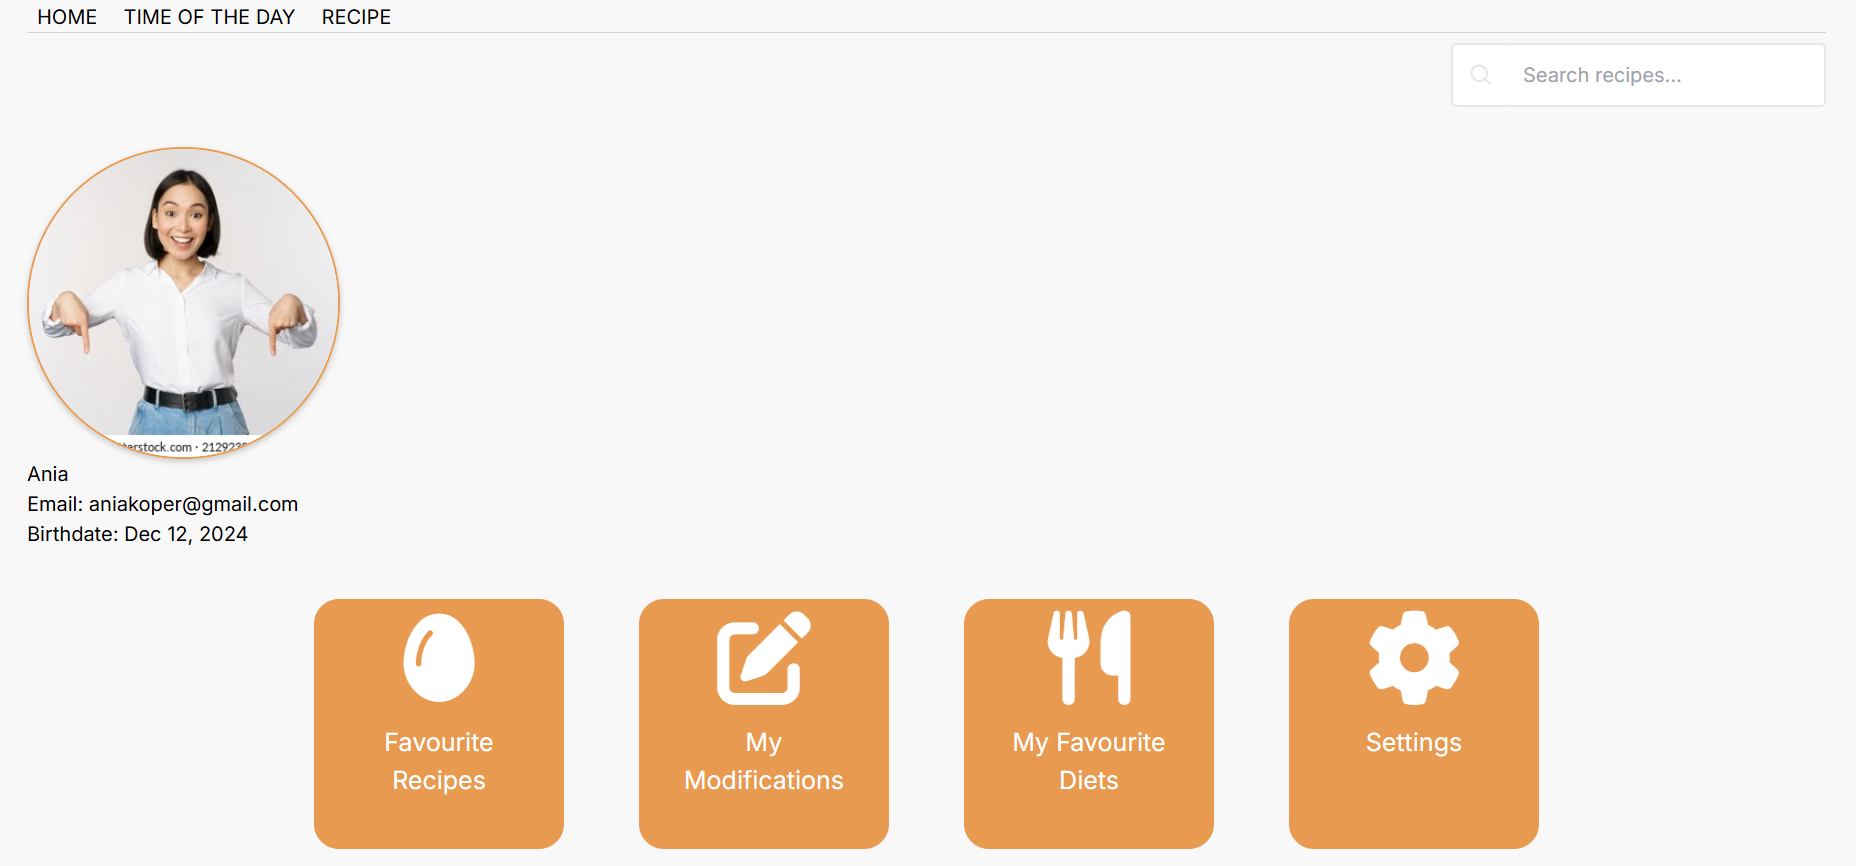
\includegraphics[width=\textwidth]{meta/pdf_attachments/images/image3.png}
    \caption{User profile}
    \label{fig:image2}
\end{figure}

5. Test Error Feedback (Optional Negative Scenarios): Enter invalid email or password and click "Login." Verify appropriate error messages are displayed. \\

\begin{figure}[H]
    \centering
    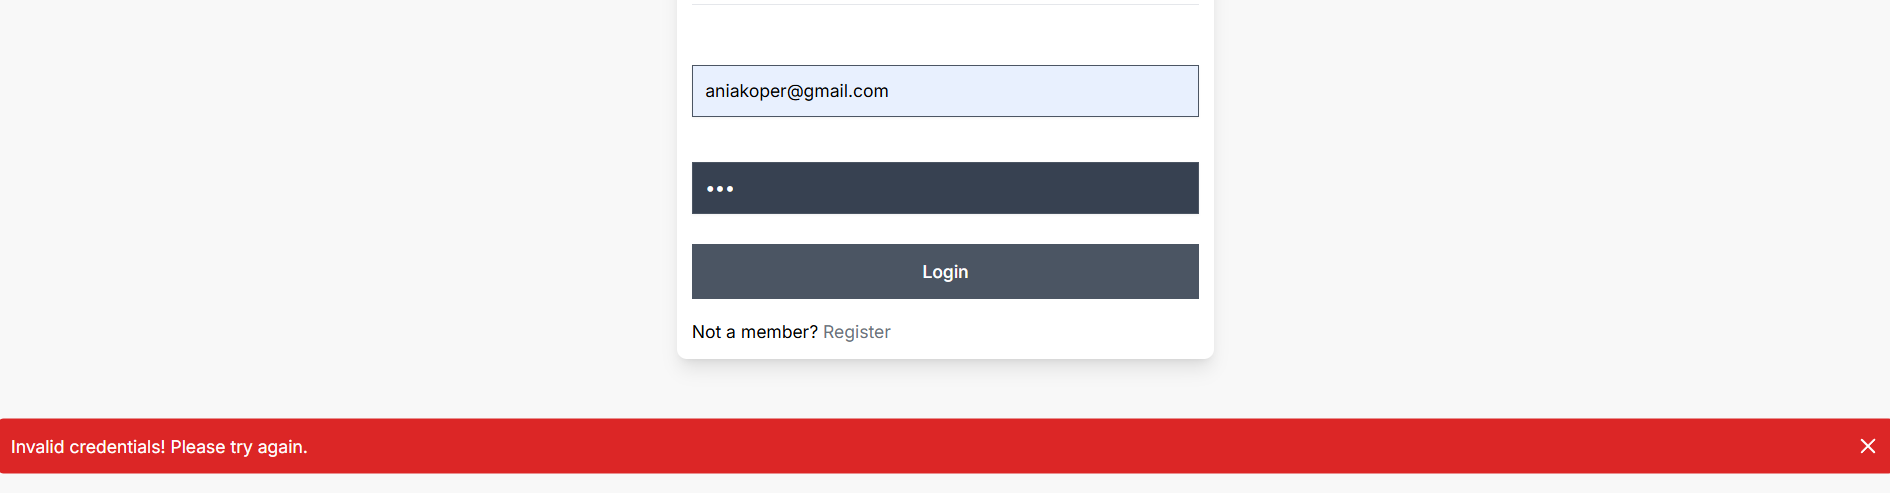
\includegraphics[width=\textwidth]{meta/pdf_attachments/images/image2.png}
    \caption{Invalid Credentials}
    \label{fig:image3}
\end{figure}

6. Session Validation: Ensure that the user remains logged in across the session unless they explicitly log out.

Expected Results: \\
- Users with valid credentials can access their personalized profile. \\
- Users with invalid credentials receive error messages. \\
- The system prevents unauthorized access to user accounts.

\subsection{Sorting and Filtering Recipes}

Objective: \\
To verify that users can effectively filter and sort recipes based on various parameters, such as diet, ingredients, calories, and ranking, and that the results are displayed correctly.

Actors Involved: \\
- End User: Anna Koper (example user) \\
- System: Foodies application

Preconditions: \\
- The user is logged into the Foodies application. \\
- The recipe database contains a variety of recipes with attributes such as dietary labels, calories, and rankings.

Test Steps: \\
1. Filtering Recipes: Navigate to the "Recipe" section and verify that the filtering options are visible. \\
   - Apply a single filter (e.g., Vegetarian) and verify that only recipes tagged as "Vegetarian" are displayed. \\
   - Apply multiple filters such as:
       - Calories: "Less than 1000 kcal." \\
     Verify that the displayed recipes satisfy all selected criteria. \\

\begin{figure}[H]
    \centering
    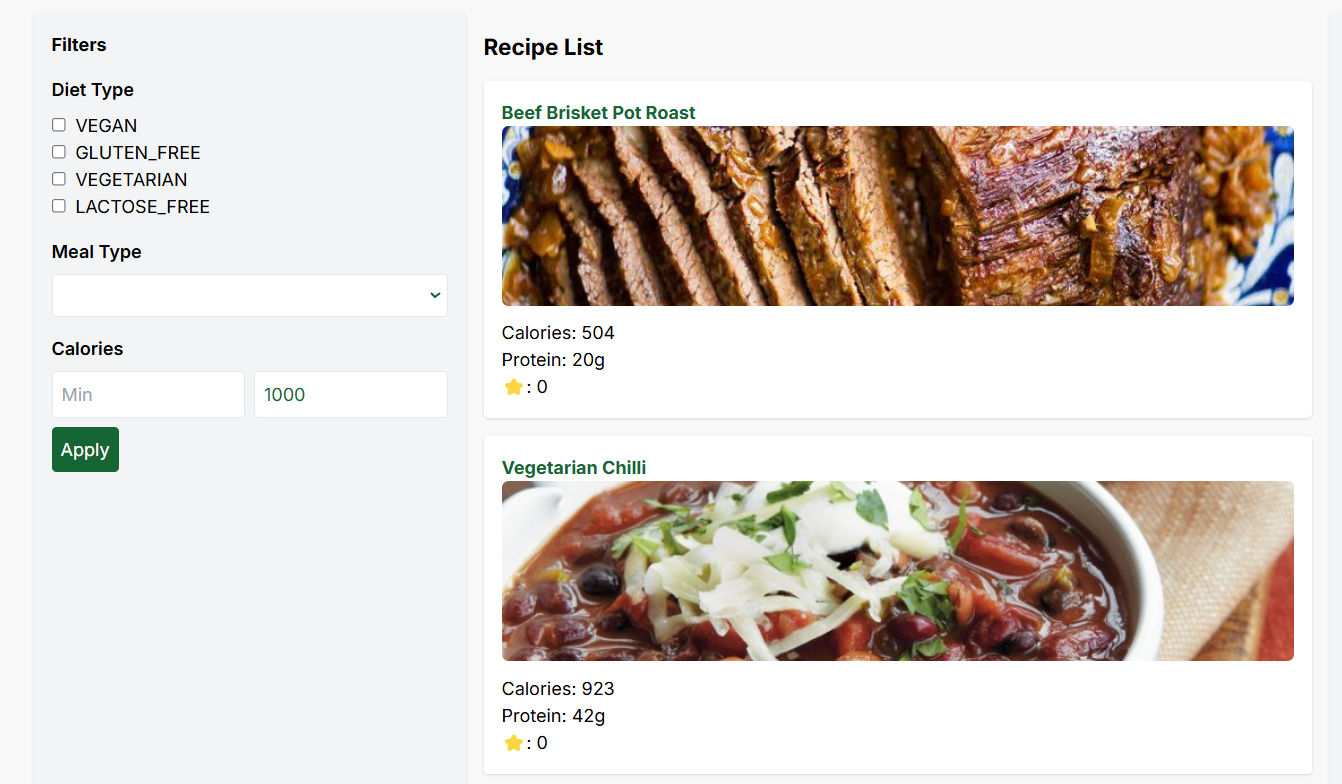
\includegraphics[width=\textwidth]{meta/pdf_attachments/images/image5.png}
    \caption{Calories filter}
    \label{fig:image4}
\end{figure}

2. Sorting Recipes: \\
   - Sort recipes by ranking (e.g., Ranking (High to Low)) and verify the results. \\
   - Sort recipes by protein content (e.g., Protein (High to Low)) and verify the results. \\

\begin{figure}[H]
    \centering
    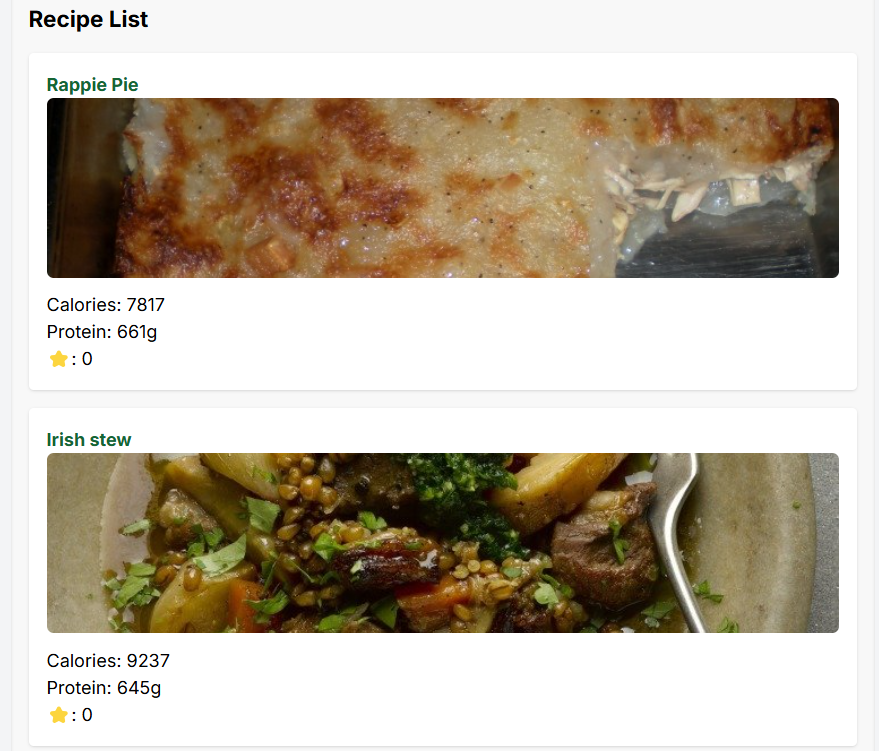
\includegraphics[width=\textwidth]{meta/pdf_attachments/images/image4.png}
    \caption{Sorted recipes - protein high to low}
    \label{fig:image5}
\end{figure}

3. Combine Sorting and Filtering: Apply a filter (e.g., Vegan) and sort the filtered results by Protein (High to Low). Verify that the recipes meet both filter and sort criteria.

\begin{figure}[H]
    \centering
    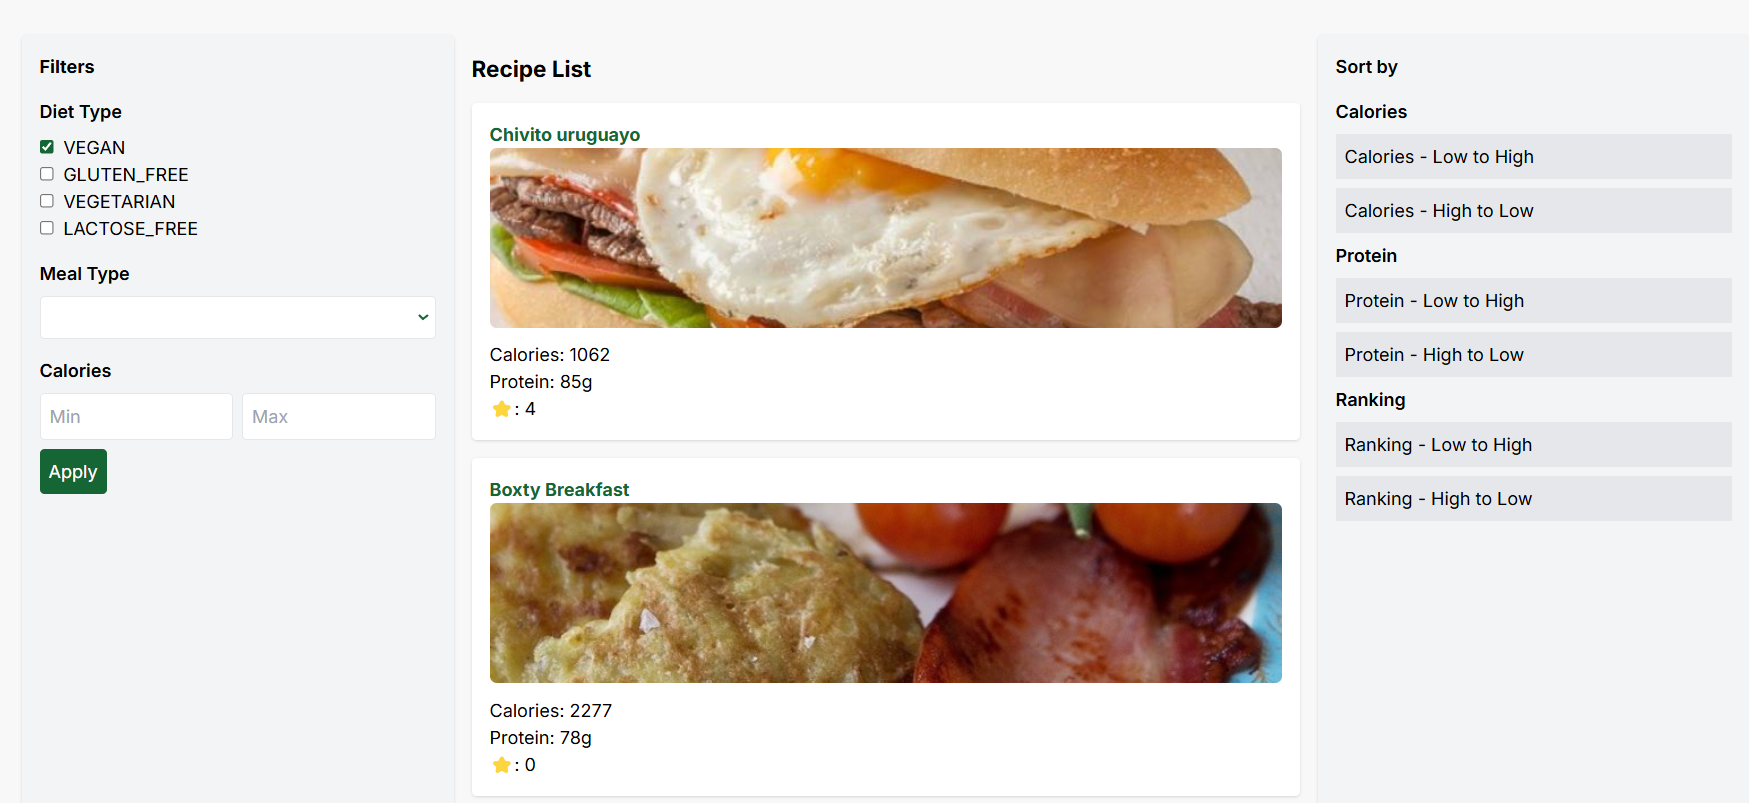
\includegraphics[width=\textwidth]{meta/pdf_attachments/images/image7.png}
    \caption{Combined filters}
    \label{fig:image6}
\end{figure}

Expected Results: \\
- Filtering criteria are applied accurately, and displayed recipes meet all selected conditions. \\
- Sorting options rearrange recipes based on the chosen attribute. \\
- Combining sorting and filtering works seamlessly.


\subsection{Substituting Ingredients in Recipes}

Objective: \\
To ensure users can substitute ingredients in recipes and verify that substitutions are accurately reflected in the recipe details.

Actors Involved: \\
- End User: Anna Koper (example user) \\
- System: Foodies application

Preconditions: \\
- The user is logged into their account on the Foodies platform. \\
- The recipe substitution functionality is enabled and accessible. \\
- The user has at least one recipe available to modify.

Test Steps: \\
1. Substitute an Ingredient: Navigate to a recipe (e.g., Chivito Uruguayo) and verify recipe details. \\
   - Click on the arrow near an ingredient to initiate substitution. \\
   - Select a substitute (e.g., gluten-free bread) and confirm. \\
   - Save the substitution and check whether the modification is saved in My Modifications. \\

\begin{figure}[H]
    \centering
    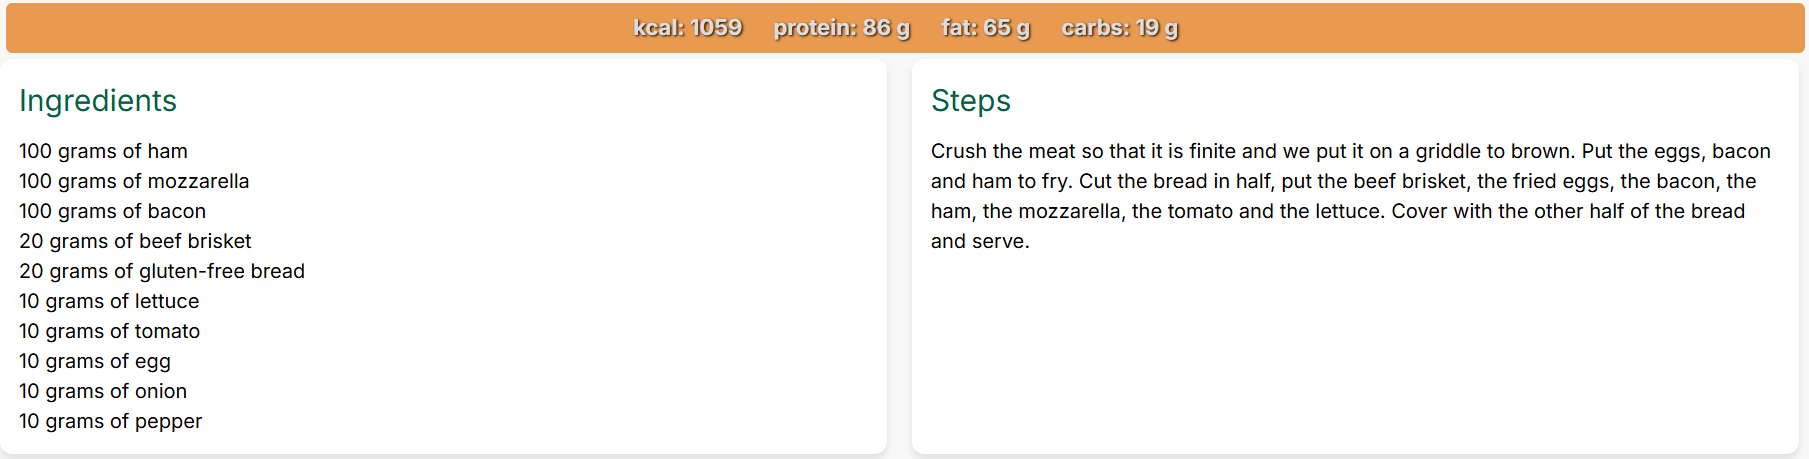
\includegraphics[width=\textwidth]{meta/pdf_attachments/images/image8.png}
    \caption{Saved Substitutions}
    \label{fig:image7}
\end{figure}

2. Edge Cases: Attempt to substitute an ingredient that has no available alternatives. \\
   - Expected Result: There is no arrow near these ingredients.

\begin{figure}[H]
    \centering
    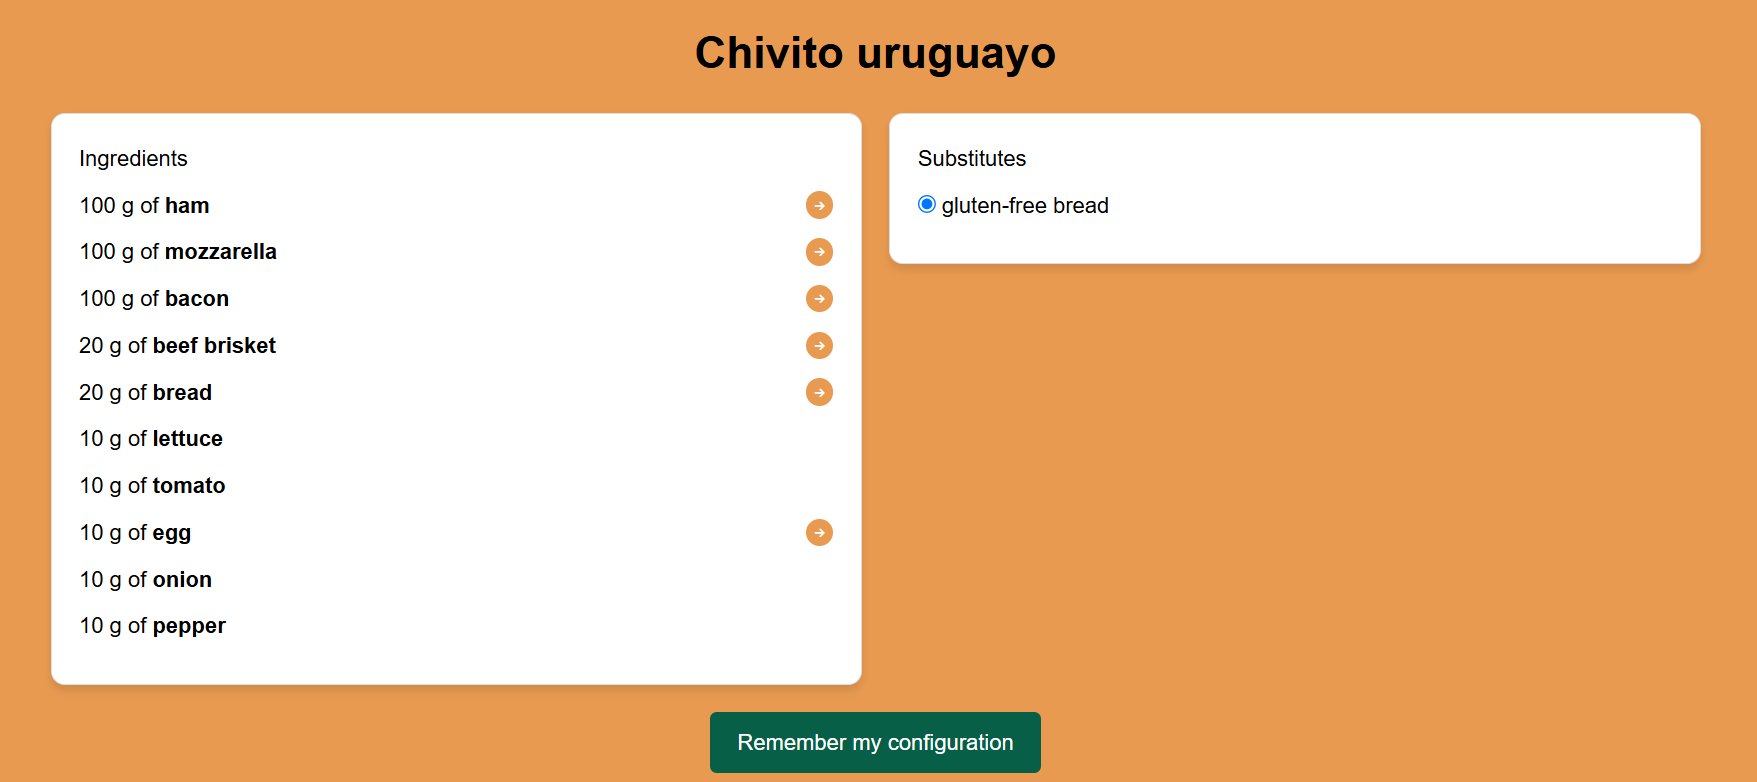
\includegraphics[width=\textwidth]{meta/pdf_attachments/images/image6.png}
    \caption{Ingredients without substitutes}
    \label{fig:image8}
\end{figure}

Expected Results: \\
- Users can substitute ingredients easily from a list of compatible options. \\
- The system reflects updated ingredient details and nutritional values after substitution. \\
- Users can revert substitutions without issues. \\
- Substitution suggestions are contextually appropriate.
